We have defined a range of clinically relevant frequencies, therefore we run a modal analysis to make sure the device is well-behaved for those frequencies.
Natural frequencies depend on an object's geometry, so the first mode of vibration we observe at \SI{934}{Hz} is only relevant to the stem length chosen.
For a \SI{16}{cm} stem we saw the first mode at \SI{670}{Hz} and for \SI{8}{cm} stem, a first mode of \SI{1668}{Hz}.
Despite all of them being above the clinically relevant frequencies, there is value in characterising the device approaching its resonant frequencies.
Therefore, we limit the simulations to below about 900 Hz.

% Figure \ref{fig:modal-frequencies} shows what some of modes look like in simulation
% \begin{figure} \centering
%     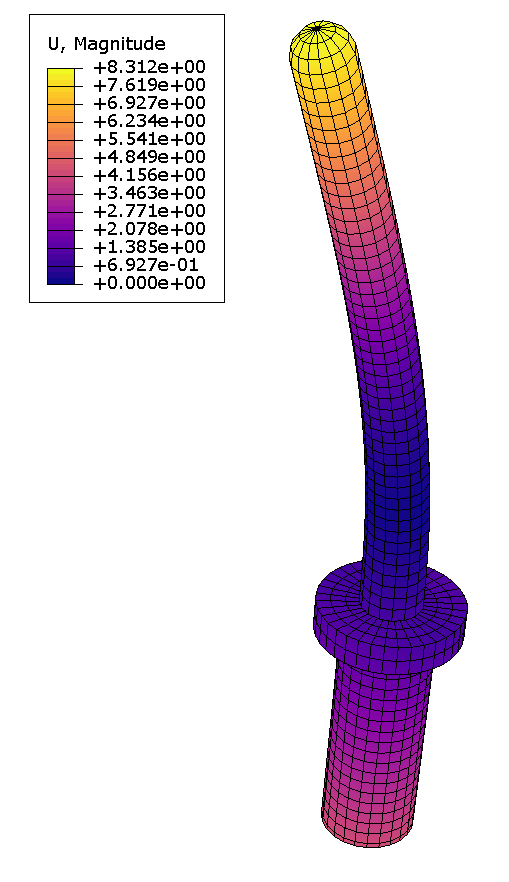
\includegraphics[height = 8cm]{figures/934.png}
%     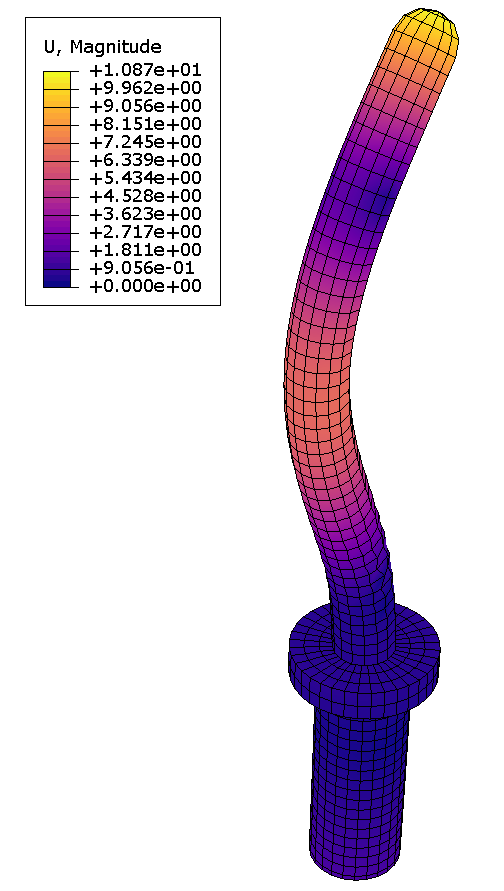
\includegraphics[height = 8cm]{figures/3933.PNG}
% \caption{Some of the modal frequencies observed for our model. Depicted are 934 Hz (left) and 3933 Hz (right). This informs the decision of keeping frequencies below the first mode.}
% \label{fig:modal-frequencies}
% \end{figure}

\paragraph{Sensor positioning}
Figure \ref{fig:10-300-900-max-displacements} shows the large variety of motion the model undergoes, which informed the decision of where the sensors have been placed.
Particularly noteworthy is one on the spigot, which contrary to initial expectations did not perfectly follow the driving force. 

\begin{figure} \centering
    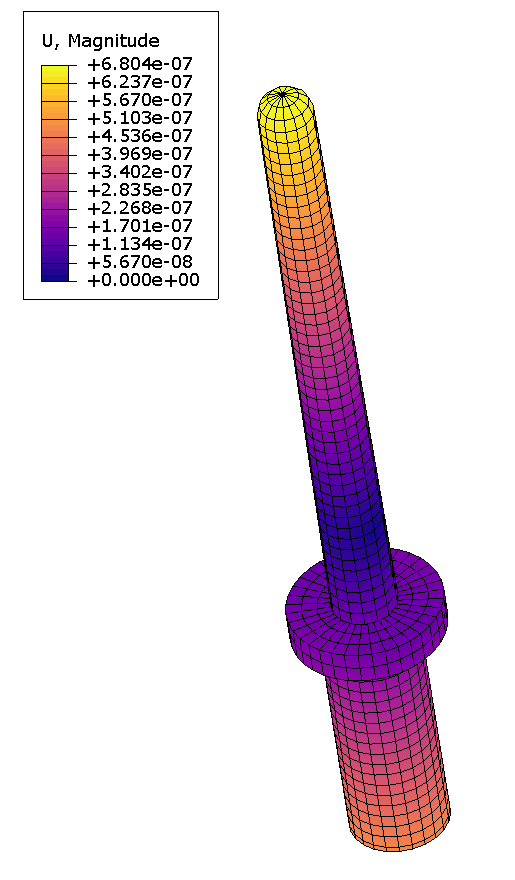
\includegraphics[width = 0.25\textwidth]{figures/Free/10hz.PNG}
    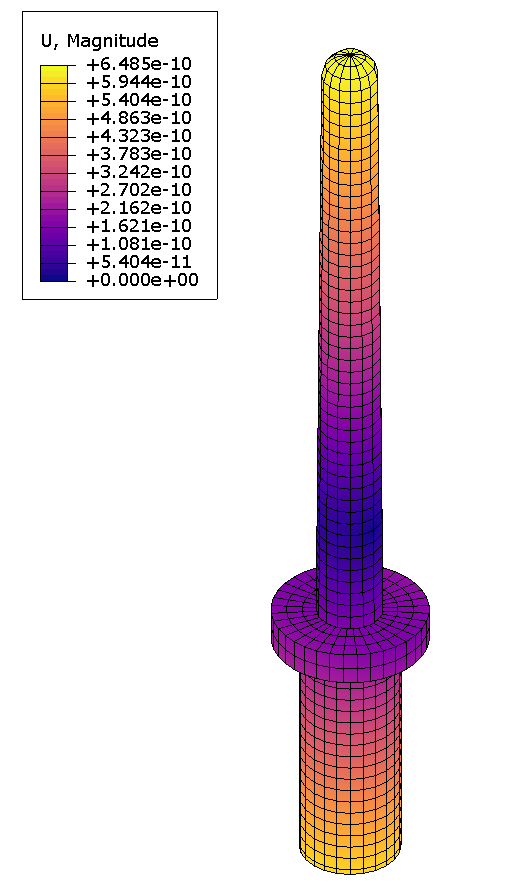
\includegraphics[width = 0.25\textwidth]{figures/Free/300hz.PNG}
    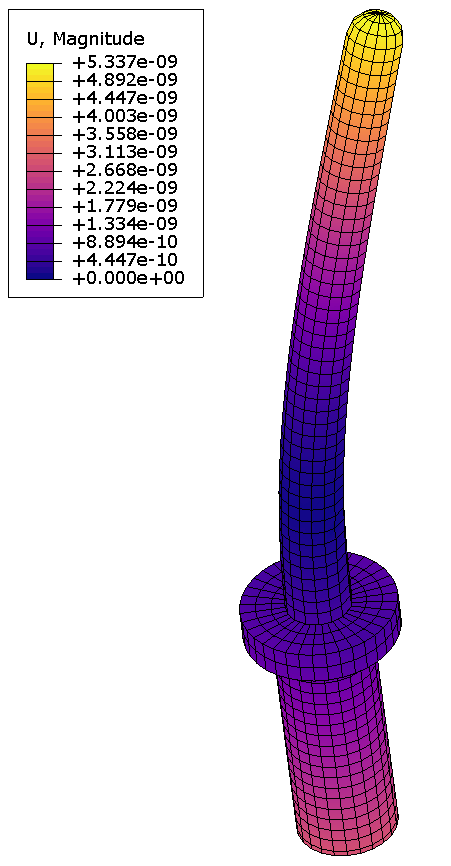
\includegraphics[width = 0.25\textwidth]{figures/Free/900hz.PNG}
\caption[Magnitude of displacement observed for 10, 300 and 900 Hz]{Magnitude of displacement observed for \SI{10}{Hz}, \SI{300}{Hz} and \SI{900}{Hz}, respectively. This highlights why we place sensors on spigot, collar and stem. Not displayed is the scaling of the deflection}
\label{fig:10-300-900-max-displacements}
\end{figure}